\documentclass[12pt]{article}
\usepackage{inputenc}
\usepackage{graphicx}
\usepackage{tabularx}
\usepackage{hyperref}

%%%%%%%%%%%%%%%%
% Impostazioni %
%%%%%%%%%%%%%%%%

\date{}

\hypersetup{
    colorlinks=true,
    linkcolor=blue,
    filecolor=magenta,
    urlcolor=cyan,
    pdftitle={Database Banca, Michael Guidelli},
    pdfpagemode=FullScreen,
}

\begin{document}

%%%%%%%%%%
% Titolo %
%%%%%%%%%%

\maketitle
\null \null \null \null \null \null
{\centering
    \huge\bfseries Database Banca \\
    \Large\normalfont Michael Guidelli  \\
}

\clearpage

%%%%%%%%%%%%%%%%%%%%%
% Traccia esercizio %
%%%%%%%%%%%%%%%%%%%%%

\section*{Traccia esercizio}

\noindent
Una banca deve gestire i dati relativi alle filiali. Per ogni filiale si devono
registrare i seguenti dati: codice, nome, città e patrimonio totale in euro.
Ogni filiale gestisce un certo insieme di conti correnti. Ogni conto
corrente è descritto dal numero del conto e dal suo saldo in euro
(positivo o negativo); ogni conto corrente può avere uno o più intestatari
(clienti), ognuno dei quali può essere intestatario di più di un conto,
anche in filiali diverse. Per ogni cliente si registrano i seguenti dati:
codice fiscale, nominativo, indirizzo, città e numero di telefono. Ogni
filiale, inoltre, concede dei prestiti ai clienti (un prestito, come un conto
corrente, può essere intestato a più di un cliente): un prestito è descritto
da un codice identificativo, dal codice del cliente a cui è stato concesso,
dal suo ammontare in euro, dal codice dell’ufficio che lo ha
concesso,dalla matricola dell’impiegato che lo ha stipulato, dalla data di
apertura e dalla data entro la quale esso dovrà essere estinto. \newline

\noindent
Dopo aver fatto le opportune ipotesi complementari elencare gli attributi
per ogni entità con relativi tipi di dato, svolgere il modelo ER e derivare il
modello logico.

\clearpage

%%%%%%%%%%%%%%%%%%%%%%%%%%%%%%%%
% Impostazioni indice e figure %
%%%%%%%%%%%%%%%%%%%%%%%%%%%%%%%%%

\renewcommand{\contentsname}{Indice \label{indice}}
\tableofcontents

\renewcommand{\listfigurename}{Lista delle figure}
\listoffigures

\renewcommand{\listtablename}{Liste Attributi}
\listoftables

\clearpage

%%%%%%%%%%%
% Ipotesi %
%%%%%%%%%%%

\section{Ipotesi}
\begin{enumerate}
    \item Ipotizzo che ogni cliente possa chiedere più di un prestito inoltre un prestito può essere cointestato.
    
    \item Essendo l'attributo nominativo un attributo atomico (attributo formato da più parti, dallo stesso tipo di dato) preferisco dividere nominativo in nome e cognome.
\end{enumerate}

%%%%%%%%%%%%%%%%%%%%%%%%%%%%%%%%%%%
% Scelta attributo identificativo %
%%%%%%%%%%%%%%%%%%%%%%%%%%%%%%%%%%%

\section{Criterio scelta attributi identificativi}

\noindent
Nella scelta degli attributi ho potuto constatare che tutte le entità eccetto l'entità Intestatario/Cliente e conto corrente, non hanno un attributo identificativo indicato dal testo, quindi ho creato degli attributi identificativi formati da numeri/lettere indicati con: id più il nome dell'entità. Nel caso dell'entità Intestatario/Cliente e conto corrente gli attributi codice fiscale e numero conto hanno le caratteristiche per essere attributi identificativi.

\clearpage

%%%%%%%%%%%%%%
% Modello ER %
%%%%%%%%%%%%%%

\section{Modello ER}
\begin{figure}[h!]
    \centering
    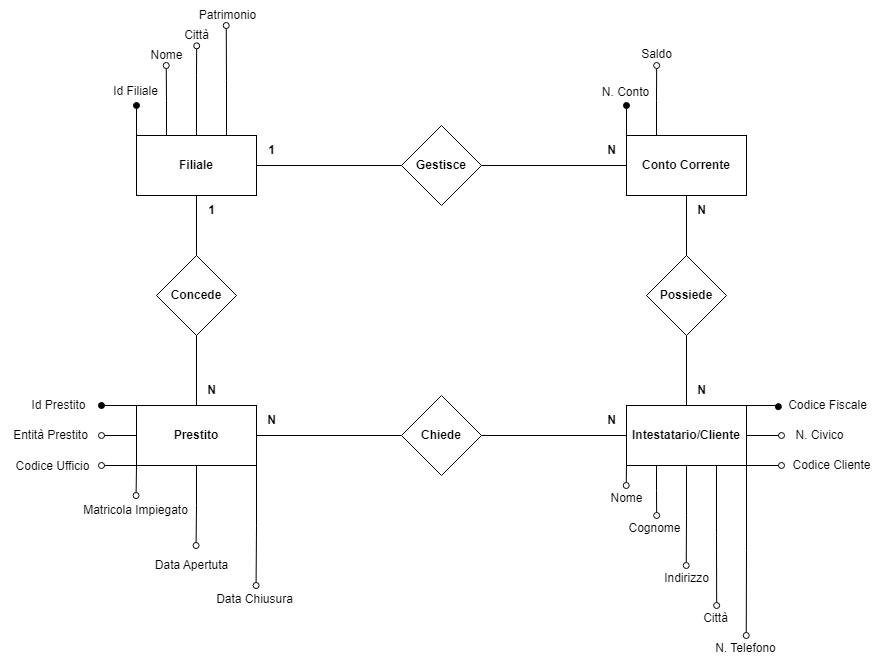
\includegraphics[width=16cm]{modello_er_banca.png}
    \label{fig:modello er}
    \caption{Rappresentazione modello ER}
\end{figure}

%%%%%%%%%%%%%%%
% Cardinalità %
%%%%%%%%%%%%%%%

\subsection{Cardinalità}

\noindent
Cardinalità delle associazioni:

\begin{itemize}
    \item \textbf{Gestisce}: in questo caso la cardinalità è \textbf{1} a \textbf{N} perché ciascuna singola filiale gestisce uno o più conti correnti e ciascun singolo conto corrente può essere gestito da una filiale.
    
    \item \textbf{Possiede}: in questo caso la cardinalità è \textbf{N} a \textbf{N} perché ciascun singolo conto corrente è posseduto da uno o più intestatari e ciascun singolo intestatario può possedere più conti correnti.
    
    \item \textbf{Concede}: in questo caso la cardinalità è \textbf{1} a \textbf{N} perché ciascuna singola filiale può concedere uno o più prestiti e ciascun singolo prestito può essere gestito da una filiale.
    
    \item \textbf{Chiede}: in questo caso la cardinalità è \textbf{N} a \textbf{N} perché ciascun singolo cliente può chiedere uno o più prestiti e ciascun singolo prestito può essere chiesto da più clienti.
\end{itemize}

\clearpage

%%%%%%%%%%%%%%%%%%%%%%%%%
% Liste degli attributi %
%%%%%%%%%%%%%%%%%%%%%%%%%

\begin{center}
    \section{Liste degli attributi}
\end{center}

% entità filiale

\subsection*{Entità Filiale}
\begin{table}[h!]
    \centering
    \begin{tabular}{|c|c|c|c|}
        \hline
        Nome attributo & Significato & Tipo di dato & Vincolo \\
        \hline
        Id filiale & Attributo identificativo & Varchar & Max 255 caratteri \\
        \hline
        Nome & Nome della filiale & Varchar & Max 255 caratteri \\
        \hline
        Città & Sede filiale & Varchar & Max 255 caratteri \\
        \hline
        Patrimonio & Complesso dei beni & Float & \\
        \hline
    \end{tabular}
    \label{tab: entità filiale}
    \caption{Lista Filiale}
\end{table}

% entità filiale 

\subsection*{Entità Conto Corrente}
\begin{table}[h!]
    \centering
    \begin{tabular}{|c|c|c|c|}
        \hline
        Nome attributo & Significato & Tipo di dato & Vincolo \\
        \hline
        Numero conto & Attributo identificativo & Varchar & Max 255 caratteri \\
        \hline
        Saldo & Saldo del conto & Float & \\
        \hline
    \end{tabular}
    \caption{Lista Conto Corrente}
    \label{tab:my_label}
\end{table}

% entità intestatario 

\subsection*{Entità Intestatario/Cliente}
\begin{table}[h!]
    \centering
    \begin{tabular}{|c|c|c|c|}
        \hline
        Nome attributo & Significato & Tipo di dato & Vincolo \\
        \hline
        Codice fiscale & Attributo identificativo & Varchar & Max 255 caratteri \\
        \hline
        Nome & Nome intestatario & Varchar & Max 255 caratteri \\
        \hline
        Cognome & Cognome intestatario & Varchar & Max 255 caratteri \\
        \hline
        Indirizzo & Indirizzo intestatario & Varchar & Max 255 caratteri \\
        \hline
        Città & Residenza intestatario & Varchar & Max 255 caratteri \\
        \hline
        Numero civico & Civico intestatario & Int & Max 3 cifre \\
        \hline
        Telefono & N.telefono intestatario & Varchar & Max 255 caratteri \\
        \hline
        Codice Cliente & Codice del cliente & Varchar & Max 255 caratteri \\
        \hline
    \end{tabular}
    \caption{Lista Intestatario/Cliente}
    \label{tab:my_label}
\end{table}

% entità prestito 

\subsection*{Entità Prestito}
\begin{table}[h!]
    \centering
    \begin{tabular}{|c|c|c|c|}
        \hline
        Nome attributo & Significato & Tipo di dato & Vincolo \\
        \hline
        Id prestito & Attributo identificativo & Varchar & Max 255 caratteri \\
        \hline
        Entità prestito & Valore del prestito & Float & \\
        \hline 
        Codice ufficio & ufficio che concede il prestito & Varchar & Max 255 caratteri \\
        \hline
        Matricola impiegato & Impiegato che stipula il prestito & Varchar & Max 255 caratteri \\
        \hline
        Data apertura & Apertura del prestito & Date & \\
        \hline 
        Data chiusura & Chiusura del prestito & Date & \\
        \hline
    \end{tabular}
    \caption{Lista Prestito}
    \label{tab:my_label}
\end{table}

\end{document}